\section{Collecting Data}
\label{sec:collecting-data}
In order to build a system to transcribe beatboxing by the common man we had to gather a dataset so base our system on. This dataset consists of the three different sounds described above, performed by several participants. The place in which we collected the data was at the Aalborg University campus in Copenhagen. In the main hall of the main building random people passing by were asked to help us out. The participants were placed in a chair surrounded by small movable walls (see figure \ref{data-collection-pic}) to limit some noise from the surroundings. They were asked in order to produce 5-10 of each of the three sounds finishing off with a short self-improvised mix of the sounds.

To record the beatboxing sequences we used a e815-S dynamic cardioid microphone attached to an H4n portable recorder. The sampling rate were at 96 kHz and 24 bits.

The data gathered has been collected as one big sound file used as a database for our system. In order to utilize this database the sound file had to be manually annotated. This means that for each sound a note had to be saved about its starting point and duration in the sound file and the type of sound. This was done using Sonic Visualiser\footnote{\url{http://www.sonicvisualiser.org/}}, which generated a text file with the needed information.

\begin{figure}[h]
	\begin{center}
		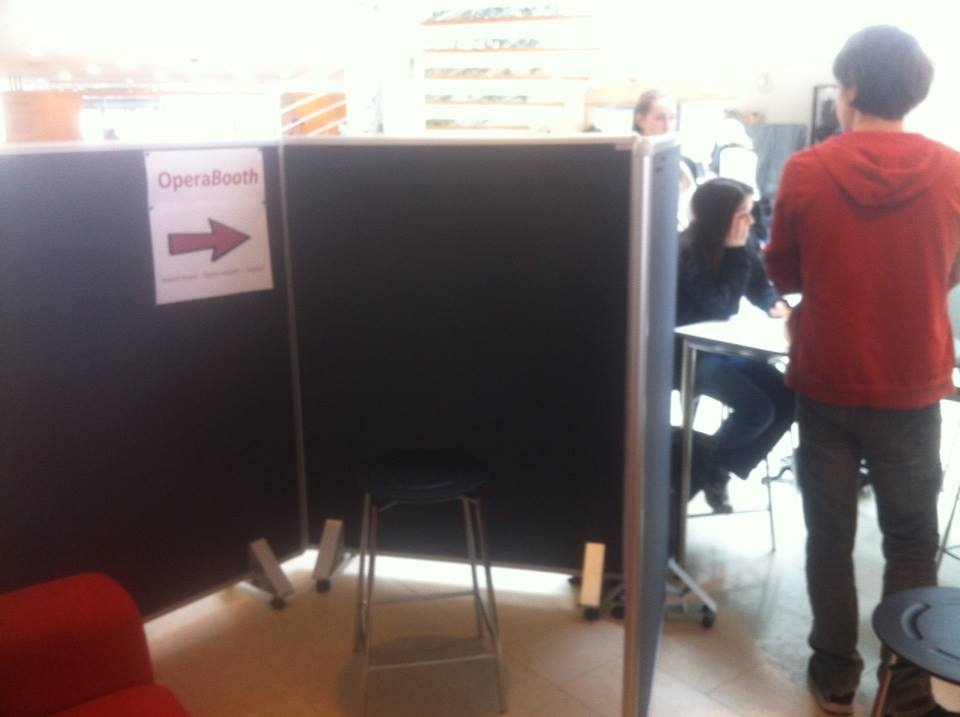
\includegraphics[height=5cm]{fig/dataset_collection.JPG}
		\caption{Data collection setup. In the image the chair on which the participants sat can be seen.}
		\label{data-collection-pic}
	\end{center}
\end{figure}